%26/10/22
Nucleo di Dirichlet
$$
D_N(\nu) = e^{-j\pi\nu(N-1)}\frac{\sin(\pi\nu N)}{\sin(\pi\nu)}
$$
Si ricava il grafico del modulo

\begin{figure}[h]
\centering
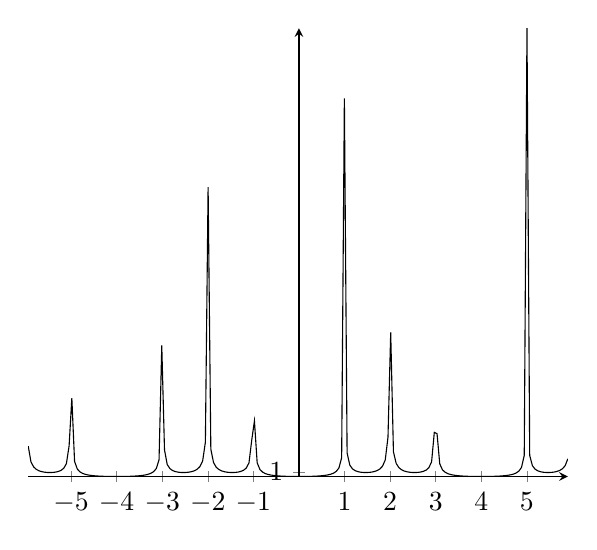
\begin{tikzpicture}
    \begin{axis}[
    axis lines = middle,
    ytick = {0,1},
    xtick = {-6,-5,...,6},
 %   xticklabels = {$-\pi$},
    %ymax = 1.1,
    ]

\addplot[domain=-6:5.9,samples=200]{abs(sin(deg(pi*x/4))/sin(deg(pi*x)))};
     % \addplot[domain=0.1:4,samples=200,grey]{1/pi/x};
     % \addplot[domain=-6:6,samples=200]{-1/pi/x};
    \end{axis}
  \end{tikzpicture}
  \caption{Funzione $D_N(x)$}
\end{figure}

Il campionamento del segnale potrebbe non avvenire in prossimità del picco di
$D_N$



Condizione di campionamento coerente, è una condizione di campionamento
sincrono particolarmente forte, sincrono significa che la frequenza di
campionamento è agganciata alla frequenza del segnale.

$\frac{f_0}{f_s} = \nu_0 = \frac{l}{N}\frac{T_s}S{T_a}$

Si è dunque in grado di scomporre frequenze e ampiezze delle componenti
contenuti nel segnale,



L'indice $l$ del bin conta quanti cicli del segnale rientrano nella finestra di
misura

In un segnale di rete, oltre alla distorsione armonica potrebbe esserci una
riduzione di power quality, ovvero dei contenuti spettrali non armonici, in tal
caso l'analisi spettrale è più difficile.

Vanno ridotti gli errori di polarizzazione e l'errore di scalop-loss.



\section{Algoritmo di Buneman}
Serve a contrastare l'errore di polarizzazione nella frequenza di una riga
spettrale, consente di compensare l'errore, dà un risultato esatto nel caso di
segnali analitici del tipo
$$
e^{j2\pi\nu_0n}
$$
con $l-1/N<\nu_0<l/N$

$$
\nu_0 = \frac{l}{N} - \frac{1}{\pi}\tan^{-1}\left(
\frac{\sin(\frac{\pi}{N})}{\cos(\frac{\pi}{N}) +
\left|\frac{X(l)}{X(l-1)}\right|}\right)
$$

Applicando la DFT al segnale analitico
$$
|X(l)|=\frac{|\sin(\pi(\frac{l}{N}-\nu_0)N)|}{|\sin(\pi(\frac{l}{N}-\nu_0)|}
$$



